%\VignetteIndexEntry{FunciSNP Vignette}
%\VignetteDepends{FunciSNP}
%\VignetteKeywords{SNP}
%\VignetteKeywords{Functional}
%\VignetteKeywords{GWAS}
%\VignettePackage{FunciSNP}
%%%%%%%%%%%%%%%%%%%%%%%%%%%%%%%%%%%%%%%%%%%%%%
\documentclass[12pt,fullpage]{article}
\usepackage{amsmath,epsfig,fullpage}
\usepackage{hyperref}
\usepackage{url}
\usepackage[authoryear,round]{natbib}
%\usepackage[OT1]{fonitenc}
\usepackage{Sweave}
%%%%%%%%%%%%%%%%%%%%%%%%%%%%%%%%%%%%%%%%%%%%%%
\newcommand{\Rfunction}[1]{{\texttt{#1}}}
\newcommand{\Robject}[1]{{\texttt{#1}}}
\newcommand{\Rpackage}[1]{{\textit{#1}}}
\newcommand{\Rclass}[1]{{\textit{#1}}}
\newcommand{\Rmethod}[1]{{\textit{#1}}}
%%%%%%%%%%%%%%%%%%%%%%%%%%%%%%%%%%%%%%%%%%%%%%
\author{Simon G. Coetzee$^\ddagger$\footnote{scoetzee@gmail.com}, Suhn
Rhie$^\ddagger$, Gerhard A. Coetzee$^\ddagger$ and Houtan
Noushmehr$^\ddagger$\footnote{houtana@gmail.com}}
%%%%%%%%%%%%%%%%%%%%%%%%%%%%%%%%%%%%%%%%%%%%%%
\begin{document}

\title{Using the FunciSNP package\\`Functional Identification of SNPs with\\
Phenotype by Coincidence with Chromatin Biofeatures'}
\maketitle

%%% Affiliation %%%
\begin{center}$^\ddagger$Norris Cancer Center\\Keck School of
Medicine\\University of Southern California\\Los Angeles, CA,
USA
\end{center}
%%%%%%%%%%%%%%%%%%%%%%%%%%%%%%%%%%%%%%%%%%%%%%
\tableofcontents
%%%%%%%%%%%%%%%%%%%%%%%%%%%%%%%%%%%%%%%%%%%%%%
%%%%%%%%%%%%%%%%%%%%%%%%%%%%%%%%%%%%%%%%%%%%%%
\section{Introduction}
%%%%%%%%%%%%%%%%%%%%%%%%%%%%%%%%%%%%%%%%%%%%%%
%%%%%%%%%%%%%%%%%%%%%%%%%%%%%%%%%%%%%%%%%%%%%%

FunciSNP assist in identifying putative functional SNP from previously
identified GWAS SNPs (tagSNP). Using information from the 1000 genomes database
as well as known position of GWAS tagSNP currated for a particular trait or
disease, FunciSNP integrates the two data along with sequence information
provided by peaks identified from high-throughput sequencing. FunciSNP assumes
user will provide peaks identified using any available ChIP peak algorithm, such
as FindPeaks.

It will identify correlated SNPs which are in linkage disequilibrium (LD) to a
known disease associated tagSNP. It will also determine if the correlated SNP in
LD to the tagSNP overlaps a genomic biological feature. Correlated SNPs are
directly imported from the current public release of the 1000 genomes database.
1000 genomes ftp servers available for the 1000 genomes public data: 

\begin{itemize}
\item National Center for Biotechnology Information
(NCBI)\footnote{\url{ftp://ftp-trace.ncbi.nih.gov/1000genomes/}}
\item European Bioinformatics Institute
(EBI)\footnote{\url{ftp://ftp.1000genomes.ebi.ac.uk/vol1/}}
\end{itemize}

Correlated SNPs in LD to a tagSNP and overlapping genomic biological features
are known as putative functional SNPs (also defined as 'FuncySNP' elsewhere in
the package).

This vignette provides a 'HOW-TO' guide to setup and run FunciSNP on your
machine. FunciSNP was developed with the idea that a user will have uninterupted
high-speed internet access as well as a desktop machine with  more than 4
multiple cores. If user is using a windows machine, multiple cores options will
not work and thus total time to complete initial FunciSNP analysis will take
longer than expected. Be sure you have uninterupted computing power when using a
windows machine. If using a linux machine, please use 'screen' (see man screen
for more information).

Using a 64bit Linux machine running 11.04 Ubuntu OS with 24G RAM and 8 cores
connected to a academic high-speed internet port, the amount of time to complete
99 tagSNP across 20 different biofeatures took less than 30 min to complete. We
anticipate about 2 hours to complete the same analysis using one core.

\subsection{GWAS SNP}
Something about GWAS SNP goes here.

\subsection{1000 genomes project}
Something about the 1000GP aims and initiative goes here. 

\subsection{Genomic features}
Something about peak calling and available data (public/private).

%%%%%%%%%%%%%%%%%%%%%%%%%%%%%%%%%%%%%%%%%%%%%%
%%%%%%%%%%%%%%%%%%%%%%%%%%%%%%%%%%%%%%%%%%%%%%
\section{Installing and Loading FunciSNP}
%%%%%%%%%%%%%%%%%%%%%%%%%%%%%%%%%%%%%%%%%%%%%%
%%%%%%%%%%%%%%%%%%%%%%%%%%%%%%%%%%%%%%%%%%%%%%

There are two options available to obtain a copy of \Rpackage{FunciSNP}: 

\begin{itemize}
\item Download current source code from Coetzeesq's
lab\footnote{\url{http://coetzeeseq.usc.edu/publication/Coetzee_SG_et_al_2012/}}
\item Download and install from
Bioconductor\footnote{\url{http://www.bioconductor.org}}
\end{itemize}

If you download the source code from either method above, you can install
\Rpackage{FunciSNP} by typing the following in your favorite unix terminal. If
you are using a non-unix terminal, please visit R CRAN for more guidance on how
to install a package from source.

By installing \Rpackage{FunciSNP} from source, the package assumes you have all
the required libraries installed.

The following loads the \Rpackage{FunciSNP} library in R.

\begin{Schunk}
\begin{Sinput}
> options(width=80);
> library(FunciSNP);
> package.version("FunciSNP");
\end{Sinput}
\begin{Soutput}
[1] "0.1.8"
\end{Soutput}
\end{Schunk}

%%%%%%%%%%%%%%%%%%%%%%%%%%%%%%%%%%%%%%%%%%%%%%
%%%%%%%%%%%%%%%%%%%%%%%%%%%%%%%%%%%%%%%%%%%%%%
\section{Running FuncySNP to identify putative functional SNPs}
%%%%%%%%%%%%%%%%%%%%%%%%%%%%%%%%%%%%%%%%%%%%%%
%%%%%%%%%%%%%%%%%%%%%%%%%%%%%%%%%%%%%%%%%%%%%%

Before we can run FuncySNP, we will need two input files. A list of tagSNp and a
folder with all available biological features (peak files in BED format).

\subsection{Create a GWAS SNP file}

GWAS SNPs (tagSNP) should be listed in a tab or whitespace separated file. Three
columns are required for each tagSNP: 

\begin{itemize}
\item Position (chrom:position)
\item rsID (rsXXXXXXXX)
\item population (EUR, AFR, AMR, ASN, or ALL)
\end{itemize}

`Positon' should be the exact postion for each rsID as reported by human genome
build hg19 (chrom:postion). `rsID' should contain a unique rsID as determined by
the 1000 genomes database (1000GP)\footnote{Be sure the rsID is located in this
browser: \url{http://browser.1000genomes.org/}} for each identified `tagSNP'.
Population should be a three letter code to determine original ethnic population
for which the associated `tagSNP' was identified. The three letter code should
be either European (EUR), Asian (ASN), African (AFR), American (AMR), or All
(ALL). List each tagSNP per ethnic population. If similar rsID was identified in
multiple ethnic population, list each duplicate tagSNP separately with the
appropriate ethnic pouplation.

As an example, we collected several GWAS SNPs significantly associated with
Glioblastoma multiforme (GBM)\footnote{See
\url{http://www.snpedia.com/index.php/Glioma}}. GBM is a brain cancer with
median survival at less than 12 months, making this form of cancer one of the
most aggressive of all cancer types. In this example, GBM includes lower grade
glioma, therefore we use the 'glioma' to label all objects.

\begin{Schunk}
\begin{Sinput}
> ## Full path to the example GWAS SNP regions file for Glioblastoma 
> #  (collected from SNPedia on Jan 2012)
> glioma.snp <- file.path(system.file('extdata', package='FunciSNP'), 
+ dir(system.file('extdata',package='FunciSNP'), pattern='.snp$'));
> gsnp <- read.delim(file=glioma.snp,sep=" ",header=FALSE);
> gsnp;
\end{Sinput}
\begin{Soutput}
            V1        V2  V3
1 11:118477367  rs498872 EUR
2    5:1286516 rs2736100 ASN
3   9:22068652 rs4977756 EUR
4  20:62309839 rs6010620 EUR
\end{Soutput}
\end{Schunk}

Now, \Robject{glioma.snp} contains the full path to the GWAS tagSNP. 

\subsection{Biofeatures in BED format}

Each biofeature used to identify correlated SNP should be in standard BED
format\footnote{See UCSC FAQ: \url{http://genome.ucsc.edu/FAQ/FAQformat}}. Each
biofeature should be stored in one folder and should have file extension
`*.bed'.

Here is an example of three different biofeatures used for this glioma example.
NRSF and PolII (both transcription factors) where extracted from a recent
release of ENCODE, as well as promoters of approximately 38,000 gene
transcription start sites (TSS). Promoters are identified as +1000 to -100 base
pair of each annotated TSS.

\begin{Schunk}
\begin{Sinput}
> ## Full path to the example biological features BED files 
> #  derived from the ENCODE project for Glioblastoma U-87 cell lines.
> glioma.bio <- system.file('extdata',package='FunciSNP');
> as.matrix(list.files(glioma.bio, pattern='.bed$'));
\end{Sinput}
\begin{Soutput}
     [,1]                    
[1,] "knownGene.TSS.hg19.bed"
[2,] "TFBS_Nrsf_U87.bed"     
[3,] "TFBS_Pol2_U87.bed"     
\end{Soutput}
\begin{Sinput}
> nrsf.filename <- list.files(glioma.bio, pattern='.bed$')[2];
> pol2.filename <- list.files(glioma.bio, pattern='.bed$')[3];
> prom.filename <- list.files(glioma.bio, pattern='.bed$')[1];
> Nrsf <- read.delim(file=paste(glioma.bio, nrsf.filename,sep="/"), sep="\t",
+ header=FALSE);
> PolII <- read.delim(file=paste(glioma.bio, pol2.filename,sep="/"), sep="\t",
+ header=FALSE);
> Promoters <- read.delim(file=paste(glioma.bio, prom.filename,sep="/"), sep="\t",
+ header=FALSE);
> dim(Nrsf);
\end{Sinput}
\begin{Soutput}
[1] 1264    6
\end{Soutput}
\begin{Sinput}
> dim(PolII);
\end{Sinput}
\begin{Soutput}
[1] 10918     6
\end{Soutput}
\begin{Sinput}
> dim(Promoters);
\end{Sinput}
\begin{Soutput}
[1] 39701     6
\end{Soutput}
\begin{Sinput}
> ## Example of what the BED format looks like:
> head(Nrsf);
\end{Sinput}
\begin{Soutput}
    V1        V2        V3                      V4 V5 V6
1 chr5 178601706 178602140 Merged-chr5-178601923-1  0  +
2 chr5 178850156 178850592 Merged-chr5-178850374-1  0  +
3 chr5 179015119 179015553 Merged-chr5-179015336-1  0  +
4 chr7     23844     24636     Merged-chr7-24240-1  0  +
5 chr7     65601     66065     Merged-chr7-65833-1  0  +
6 chr7    128907    129421    Merged-chr7-129164-1  0  +
\end{Soutput}
\end{Schunk}

As an example, \Robject{Nrsf} was created to illustrate the format needed for
each biofeatures. To run FuncySNP, only the path to the folder to each
biofeature is required (\Robject{glioma.bio}.

\subsection{FuncySNP analysis using two inputs}

To run the example data could take more than 5 minutes, thus the R code is
commented out for this tutorial. If you are interested in running the glioma
example from scratch, please uncomment the following and rerun in your R
session. (The main function of FunciSNP is \Rmethod{FuncySNP}.)

\begin{Schunk}
\begin{Sinput}
> ## FunciSNP analysis, extracts correlated SNPs from the 
> #  1000 genomes db ("ncbi" or "ebi") and finds overlaps between 
> #  correlated SNP and biological features and then 
> #  calculates LD (Rsquare, Dprime, distance, p-value).
> ## Depending on number of CPUs and internet connection, this step may take 
> # some time. Please consider using a unix machine to access multiple cores.
> # glioma <- FuncySNP(snp.regions.file=glioma.snp, 
> #           bio.features.loc = glioma.bio, 
> #           bio.features.TSS=FALSE);
> # glioma;
> # summary(glioma);
\end{Sinput}
\end{Schunk}

As an alternative, \Robject{glioma} was pre-run and stored in the package as an
R object. To call this data object, simily run the following commands. 

\begin{Schunk}
\begin{Sinput}
> data(glioma);
> class(glioma);
\end{Sinput}
\begin{Soutput}
[1] "TSList"
attr(,"package")
[1] "FunciSNP"
\end{Soutput}
\end{Schunk}

Now, \Robject{glioma} contains the R data structure that holds all the results
for this particular analysis. Each tagSNP is stored as a slot which contains
associated correlated SNP and overlapping biofeature. It also contains a number
of different annotations (see below for more details). To see a brief summary of
the results (\Rmethod{summary}), type the following commands:

\begin{Schunk}
\begin{Sinput}
> glioma;
\end{Sinput}
\begin{Soutput}
TagSNP List with  4  Tag SNPs and 
 778 nearby,  potentially correlated SNPs, that overlap at least one biofeature 
$`R squared: 0.1`
             Total R.squared.cuff.0.1 Percent
tagSNPs          4                  3   75.00
1kSNPs         778                 64    8.23
bio.features     3                  3  100.00

$`R squared: 0.5`
             Total R.squared.cuff.0.5 Percent
tagSNPs          4                  3   75.00
1kSNPs         778                 44    5.66
bio.features     2                  2  100.00

$`R squared: 0.9`
             Total R.squared.cuff.0.9 Percent
tagSNPs          4                  1   25.00
1kSNPs         778                 13    1.67
bio.features     2                  2  100.00
\end{Soutput}
\end{Schunk}

As you can quickly observe from the above analysis, using 4 tagSNPs position and
3 different biological features (ChIPseq for `NRSF', `PolII', promoters of
approx. 38,000 genes) as two types of input, FunciSNP identified 778 1000GP SNPs
that overlap at least one biofeature. Each 1000GP SNP contains an Rsquare value
to the associated tagSNP. As a result, the first output (\Robject{glioma}),
summarizes the analysis subsetted in three different Rsquare values (0.1, 0.5
and 0.9). If we consider Rsquare cutoff at 0.9 (Rsquare $\ge$ 0.9), 13 1000GP SNPs
overlapping at least one biofeature. This value represents 1.67\% of the total
(778). In addition, at this Rsquare cutoff, 2 biological features are
represented among the 13 1000GP SNPs.

\begin{Schunk}
\begin{Sinput}
> summary(glioma);
\end{Sinput}
\begin{Soutput}
TagSNP List with  4  Tag SNPs and 
 778 nearby,  potentially correlated SNPs, that overlap at least one biofeature 
Number of potentially correlated SNPs 
overlapping at least x biofeatures, per Tag SNP at an R squared of
$`R squared: 0.1 in 4 Tag SNPs with a total of `
                        bio.1 bio.2
rs4977756                   3     0
rs498872                    9     2
rs6010620                  52     9
TOTAL # CORRELATED SNPS    64    11

$`R squared: 0.5 in 4 Tag SNPs with a total of `
                        bio.1 bio.2
rs4977756                   2     0
rs498872                    2     0
rs6010620                  40     6
TOTAL # CORRELATED SNPS    44     6

$`R squared: 0.9 in 2 Tag SNPs with a total of `
                        bio.1
rs6010620                  13
TOTAL # CORRELATED SNPS    13
\end{Soutput}
\end{Schunk}

Running \Rmethod{summary} however will output a slightly different report yet
just as informative. At three different Rsquare cutoffs (0.1, 0.5, 0.9), the
summary output illustrates the tagSNP with the total number of 1000GP SNPs
overlapping a total number of biofeatures. For example, at Rsquare $\ge$ 0.5,
tagSNP `rs6010620' is assocated with 40 different 1000GP SNPs which overlap at
least one biofeature, and 6 of them overlap at least two biofeatures.

Each newly identified 1000GP SNP is now defined as putative functional SNP since
they are in LD to an associated tagSNP and they overlap at least one interesting
biological feature. Thus, each 1000GP SNP is now characterized as
`\textbf{Func-y-SNP}.'

%%%%%%%%%%%%%%%%%%%%%%%%%%%%%%%%%%%%%%%%%%%%%%
%%%%%%%%%%%%%%%%%%%%%%%%%%%%%%%%%%%%%%%%%%%%%%
\section{Annotating newly identified Func-y-SNPs}
%%%%%%%%%%%%%%%%%%%%%%%%%%%%%%%%%%%%%%%%%%%%%%
%%%%%%%%%%%%%%%%%%%%%%%%%%%%%%%%%%%%%%%%%%%%%%

All known genomic features (exon, intron, 5'UTR, 3'UTR, promoter, lincRNA or in
gene desert (intergentic)) are used to annotate each newly identified Func-y-SNP
as described above. Information stored in this \Robject{glioma.anno} is used for
all summary plots, table, and to output results in BED format (see following
sections for more details). The following step will output the data.frame.

\begin{Schunk}
\begin{Sinput}
> glioma.anno <- FunciSNPAnnotateSummary(glioma);
> class(glioma.anno);
\end{Sinput}
\begin{Soutput}
[1] "data.frame"
\end{Soutput}
\begin{Sinput}
> gl.anno <- glioma.anno;
> ## remove rownames for this example section.
> rownames(gl.anno) <- c(1:length(rownames(gl.anno)))
> dim(gl.anno);
\end{Sinput}
\begin{Soutput}
[1] 862  28
\end{Soutput}
\begin{Sinput}
> head(gl.anno[,c(1:18,20:28)]); ## 
\end{Sinput}
\begin{Soutput}
  chromosome bio.feature.start bio.feature.end        bio.feature  corr.snp.id
1          5           1200710         1201809 knownGene.TSS.hg19 chr5:1200720
2          5           1200710         1201809 knownGene.TSS.hg19 chr5:1200766
3          5           1200710         1201809 knownGene.TSS.hg19 chr5:1200817
4          5           1200710         1201809 knownGene.TSS.hg19 chr5:1200946
5          5           1200710         1201809 knownGene.TSS.hg19 chr5:1200976
6          5           1200710         1201809 knownGene.TSS.hg19 chr5:1201033
  corr.snp.position tag.snp.id tag.snp.position   D.prime    R.squared p.value
1           1200720  rs2736100          1286516        NA           NA       1
2           1200766  rs2736100          1286516        NA           NA       1
3           1200817  rs2736100          1286516        NA           NA       1
4           1200946  rs2736100          1286516        NA           NA       1
5           1200976  rs2736100          1286516 1.0000000 0.0022585199       1
6           1201033  rs2736100          1286516 0.1795671 0.0004069606       1
  distance.from.tag population.count population nearest.lincRNA.ID
1            -85796              286        ASN     TCONS_00010241
2            -85750              286        ASN     TCONS_00010241
3            -85699              286        ASN     TCONS_00010241
4            -85570              286        ASN     TCONS_00010241
5            -85540              286        ASN     TCONS_00010241
6            -85483              286        ASN     TCONS_00010241
  nearest.lincRNA.distancetoFeature nearest.lincRNA.coverage
1                            -39302                 upstream
2                            -39348                 upstream
3                            -39399                 upstream
4                            -39528                 upstream
5                            -39558                 upstream
6                            -39615                 upstream
  nearest.TSS.GeneSymbol nearest.TSS.ensembl nearest.TSS.coverage
1                SLC6A19     ENSG00000174358             upstream
2                SLC6A19     ENSG00000174358             upstream
3                SLC6A19     ENSG00000174358             upstream
4                SLC6A19     ENSG00000174358             upstream
5                SLC6A19     ENSG00000174358             upstream
6                SLC6A19     ENSG00000174358             upstream
  nearest.TSS.distancetoFeature Promoter utr5 Exon Intron utr3 Intergenic
1                          -990      YES   NO   NO     NO   NO         NO
2                          -944      YES   NO   NO     NO   NO         NO
3                          -893      YES   NO   NO     NO   NO         NO
4                          -764      YES   NO   NO     NO   NO         NO
5                          -734      YES   NO   NO     NO   NO         NO
6                          -677      YES   NO   NO     NO   NO         NO
\end{Soutput}
\begin{Sinput}
> names(gl.anno);
\end{Sinput}
\begin{Soutput}
 [1] "chromosome"                        "bio.feature.start"                
 [3] "bio.feature.end"                   "bio.feature"                      
 [5] "corr.snp.id"                       "corr.snp.position"                
 [7] "tag.snp.id"                        "tag.snp.position"                 
 [9] "D.prime"                           "R.squared"                        
[11] "p.value"                           "distance.from.tag"                
[13] "population.count"                  "population"                       
[15] "nearest.lincRNA.ID"                "nearest.lincRNA.distancetoFeature"
[17] "nearest.lincRNA.coverage"          "nearest.TSS.GeneSymbol"           
[19] "nearest.TSS.refseq"                "nearest.TSS.ensembl"              
[21] "nearest.TSS.coverage"              "nearest.TSS.distancetoFeature"    
[23] "Promoter"                          "utr5"                             
[25] "Exon"                              "Intron"                           
[27] "utr3"                              "Intergenic"                       
\end{Soutput}
\begin{Sinput}
> summary(gl.anno[,c(1:18,20:28)]);
\end{Sinput}
\begin{Soutput}
  chromosome        bio.feature.start   bio.feature.end    
 Length:862         Min.   :  1200710   Min.   :  1201809  
 Class :character   1st Qu.: 62295044   1st Qu.: 62295926  
 Mode  :character   Median : 62326155   Median : 62337392  
                    Mean   : 65165595   Mean   : 65169512  
                    3rd Qu.: 62374564   3rd Qu.: 62376020  
                    Max.   :118531575   Max.   :118532674  
                                                           
             bio.feature           corr.snp.id  corr.snp.position  
 knownGene.TSS.hg19:372   chr11:118442863:  2   Min.   :  1200720  
 TFBS_Nrsf_U87     : 22   chr11:118443036:  2   1st Qu.: 62295889  
 TFBS_Pol2_U87     :468   chr11:118443046:  2   Median : 62327508  
                          chr11:118478342:  2   Mean   : 65167605  
                          chr20:62289690 :  2   3rd Qu.: 62375255  
                          chr20:62289873 :  2   Max.   :118532636  
                          (Other)        :850                      
     tag.snp.id  tag.snp.position       D.prime            R.squared        
 rs2736100: 96   Min.   :  1286516   Min.   :7.835e-04   Min.   :9.520e-08  
 rs4977756: 25   1st Qu.: 62309839   1st Qu.:9.338e-01   1st Qu.:7.765e-04  
 rs498872 :166   Median : 62309839   Median :1.000e+00   Median :4.501e-03  
 rs6010620:575   Mean   : 65163135   Mean   :8.995e-01   Mean   :1.258e-01  
                 3rd Qu.: 62309839   3rd Qu.:1.000e+00   3rd Qu.:2.804e-02  
                 Max.   :118477367   Max.   :1.000e+00   Max.   :9.776e-01  
                                     NA's   :4.710e+02   NA's   :4.710e+02  
    p.value           distance.from.tag population.count population
 Min.   :2.115e-163   Min.   :-100000   Min.   :286.0    ASN: 96   
 1st Qu.: 1.000e+00   1st Qu.: -19966   1st Qu.:379.0    EUR:766   
 Median : 1.000e+00   Median :  13942   Median :379.0              
 Mean   : 7.989e-01   Mean   :   4470   Mean   :368.6              
 3rd Qu.: 1.000e+00   3rd Qu.:  25290   3rd Qu.:379.0              
 Max.   : 1.000e+00   Max.   :  67371   Max.   :379.0              
                                                                   
      nearest.lincRNA.ID nearest.lincRNA.distancetoFeature
 TCONS_00010241: 96      Min.   :-265183                  
 TCONS_00015797: 25      1st Qu.: -92280                  
 TCONS_00020001:166      Median :  59111                  
 TCONS_00027984: 26      Mean   :   2073                  
 TCONS_00028269:549      3rd Qu.:  73343                  
                         Max.   : 246019                  
                                                          
 nearest.lincRNA.coverage    nearest.TSS.GeneSymbol      nearest.TSS.ensembl
 downstream:565           TNFRSF6B      :305        ENSG00000243509:305     
 inside    :  9           PHLDB1        : 86        ENSG00000019144: 86     
 upstream  :288           ZGPAT         : 68        ENSG00000197114: 68     
                          RTEL1;TNFRSF6B: 37        ENSG00000229299: 59     
                          SLC6A18       : 34        ENSG00000026036: 37     
                          (Other)       :202        ENSG00000244977: 36     
                          NA's          :130        (Other)        :271     
 nearest.TSS.coverage nearest.TSS.distancetoFeature Promoter   utr5    
 downstream:103       Min.   :-16454.0              NO :694   NO :825  
 inside    :311       1st Qu.: -3117.0              YES:168   YES: 37  
 upstream  :448       Median :   -76.0                                 
                      Mean   :   890.4                                 
                      3rd Qu.:  2305.8                                 
                      Max.   : 28781.0                                 
                                                                       
  Exon     Intron     utr3     Intergenic
 NO :776   NO :413   NO :702   NO :810   
 YES: 86   YES:449   YES:160   YES: 52   
\end{Soutput}
\begin{Sinput}
> rm(gl.anno);
\end{Sinput}
\end{Schunk}

As you can see, each tagSNP (`tag.snp.id') is associated with an identifiable
Func-y-SNP (`corr.snp.id') and each are associated with a biological feature
(`bio.feature'). Additional columns are included which assist in summarizing the
final results.

Now, if you prefer, you can use several functions to help summarize and plot
the final analysis or you can use your own set of scripts to further summarize
the results.  Either case, the final results are stored in
\Robject{glioma.anno}.

%%%%%%%%%%%%%%%%%%%%%%%%%%%%%%%%%%%%%%%%%%%%%%
%%%%%%%%%%%%%%%%%%%%%%%%%%%%%%%%%%%%%%%%%%%%%%
\section{Summarize FunciSNP results}
%%%%%%%%%%%%%%%%%%%%%%%%%%%%%%%%%%%%%%%%%%%%%%
%%%%%%%%%%%%%%%%%%%%%%%%%%%%%%%%%%%%%%%%%%%%%%

The following sections describe methods to summarize and plot the newly
identified Func-y-SNPs.

\subsection{Summary table used to describe newly identified Func-y-SNPs}

Using a specified Rsquare value (0-1) to subset the data, a table is generated
which summarizes the total number of Func-y-SNPs, associated tagSNPs, and number
of overlapping biofeatures. This will provide user a first look at the total
number of available Func-y-SNP at a particular Rsquare cutoff.

The output is very similar to the output generated by calling \Robject{glioma}.
But instead of getting a summary report three distinct Rsquare cutoffs, you can
now specify the Rsquare cutoffs.  In this case, we used rsq=0.44.

\begin{Schunk}
\begin{Sinput}
> FunciSNPtable(glioma.anno, rsq=0.44);
\end{Sinput}
\begin{Soutput}
             Total R.squared.cuff.0.44 Percent
tagSNPs          4                   3   75.00
1kSNPs         778                  46    5.91
bio.features     2                   2  100.00
\end{Soutput}
\end{Schunk}

If `geneSum' argument is set to `TRUE', a list of gene names is reported
instead which informs on the nearest gene symbols to the set of Func-y-SNPs.
Only unique gene symbols are reported since multiple distinct Func-y-SNP can be
near the same gene.

\begin{Schunk}
\begin{Sinput}
> FunciSNPtable(glioma.anno, rsq=0.44, geneSum=TRUE);
\end{Sinput}
\begin{Soutput}
      Gene_Names
1         CDKN2B
2          LIME1
3         PHLDB1
4       SLC2A4RG
5       TNFRSF6B
6           TREH
7          ZGPAT
8 RTEL1;TNFRSF6B
\end{Soutput}
\end{Schunk}

\subsection{Summary of correlated SNPs overlapping biofeatures}

The following function (\Rmethod{FunciSNPsummaryOverlaps} helps to determine the
total number of Func-y-SNPs overlapping a number of different biofeatures. This
is similar to running \Rmethod{summary} on \Robject{glioma} above, except now
you can specifically call the function and set a pre-determined 'rsq' value to
subset the data and thereby obtain a more objective and informative result.

\begin{Schunk}
\begin{Sinput}
> FunciSNPsummaryOverlaps(glioma.anno)
\end{Sinput}
\begin{Soutput}
                        bio.1 bio.2
rs2736100                  41     0
rs4977756                  12     0
rs498872                   59     3
rs6010620                 236    40
TOTAL # CORRELATED SNPS   348    43
\end{Soutput}
\end{Schunk}

Using a 'rsq' value, the output is subsetted to summarize the results with 
Rsquare values $\ge$ 'rsq'.

\begin{Schunk}
\begin{Sinput}
> FunciSNPsummaryOverlaps(glioma.anno, rsq=0.44)
\end{Sinput}
\begin{Soutput}
                        bio.1 bio.2
rs4977756                   2     0
rs498872                    2     0
rs6010620                  42     7
TOTAL # CORRELATED SNPS    46     7
\end{Soutput}
\end{Schunk}

\subsection{Summary of correlated SNPs for a number of different tagSNPs}

After running \Rmethod{FunciSNPsummaryOverlaps}, the next question one would
like to know is which correlated SNPs overlapping a number of different
biofeatures for a number of associated tagSNP. Thus, in the example above, we
have determined that we are interested in learning more about the Func-y-SNPs
associated with 'rs6010620' and which overlap at least 2 different biofeatures.

\begin{Schunk}
\begin{Sinput}
> rs6010620 <- FunciSNPidsFromSummary(glioma.anno, tagsnpid="rs6010620",
+ num.features=2, rsq=0.44);
> #summary(rs6010620);
> dim(rs6010620);
\end{Sinput}
\begin{Soutput}
[1] 14 28
\end{Soutput}
\begin{Sinput}
> class(rs6010620);
\end{Sinput}
\begin{Soutput}
[1] "data.frame"
\end{Soutput}
\begin{Sinput}
> ## See FunciSNPbed to visualize this data in a genome browser.
\end{Sinput}
\end{Schunk}

%%%%%%%%%%%%%%%%%%%%%%%%%%%%%%%%%%%%%%%%%%%%%%
%%%%%%%%%%%%%%%%%%%%%%%%%%%%%%%%%%%%%%%%%%%%%%
\section{Plot FunciSNP results}
%%%%%%%%%%%%%%%%%%%%%%%%%%%%%%%%%%%%%%%%%%%%%%
%%%%%%%%%%%%%%%%%%%%%%%%%%%%%%%%%%%%%%%%%%%%%%

\Rmethod{FunciSNPplot} is a function developed to plot various types of plots to
summarize and assist end-user in making informed discoveries of FunciSNP
results. Plots can be stored in a folder for future reference. Most plots were
created in with the idea that they can be directly outputted in presentations or
publication formats.

The following example plots the distribution of the Rsquare values for each
Func-y-SNP (Figure \ref{fig:glioma_dist.pdf}). We recommend attempting this plot
before subsetting any data by a specified rsq value. The distribution helps to
identify a specific Rsquare value that will provide the most informative
discovery.

\begin{Schunk}
\begin{Sinput}
> pdf("glioma_dist.pdf")
> FunciSNPplot(glioma.anno)
> dev.off()
\end{Sinput}
\begin{Soutput}
null device 
          1 
\end{Soutput}
\end{Schunk}

\begin{figure}[ht!]
\begin{center}
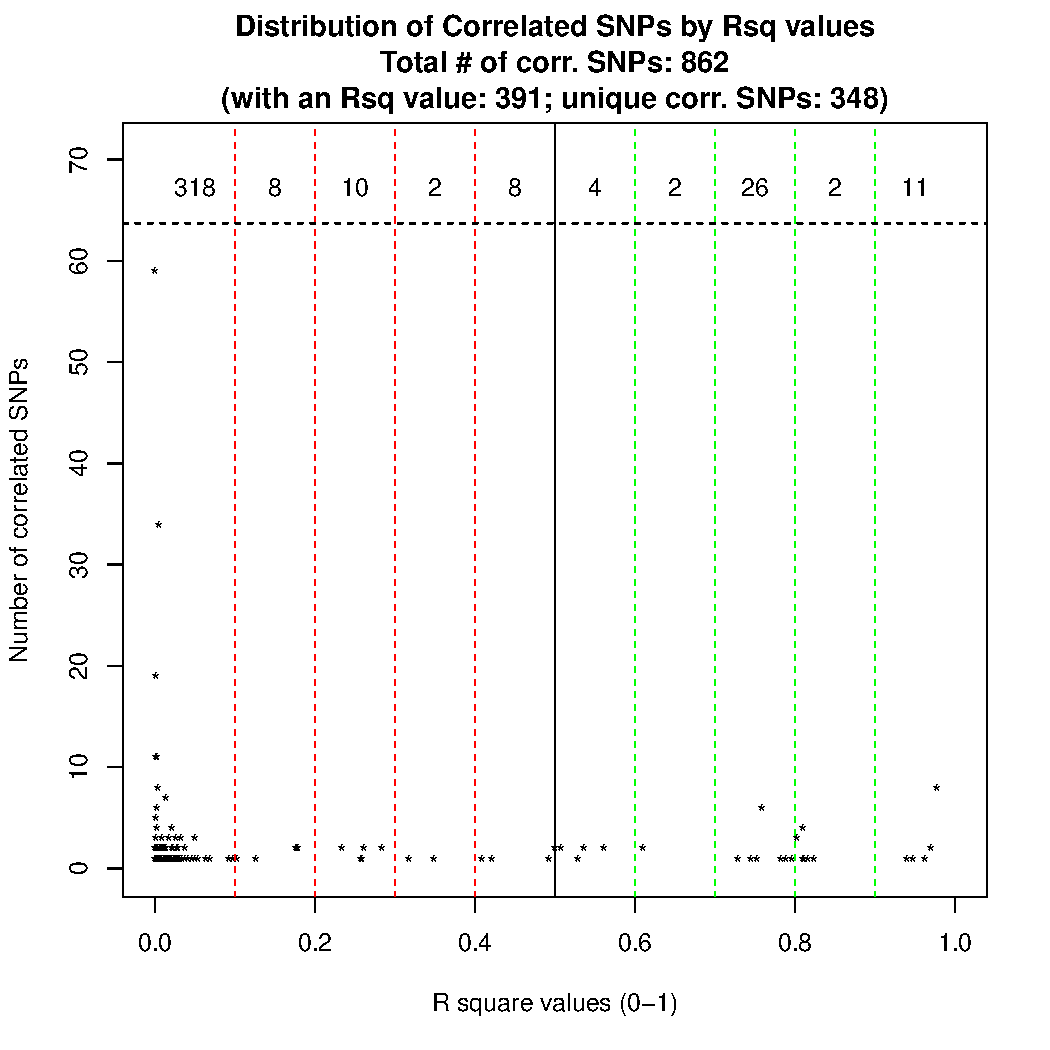
\includegraphics{glioma_dist.pdf}
\caption{\label{fig:glioma_dist.pdf} Distribution of Rsquare values of all 
Func-y-SNPs. Each marked bin contains the total number of Func-y-SNPs
(correlated SNPs). The sum of all the counts would total the number of
correlated SNPs.}
{\footnotesize{}}
\end{center}
\end{figure}

Figure \ref{fig:glioma_dist.pdf} illustrates the total number of Func-y-SNPs
binned at different Rsquare cutoffs. As you can see in this figure
(\ref{fig:glioma_dist.pdf}, there are a total of 11 Func-y-SNP with an Rsquare
$\ge$ 0.9. Since this plot does not take into consideration unique Func-y-SNP
the number may represent duplicate Func-y-SNP since they may overlap more than
one biological feature.

Using `splitbysnp' argument, the same type of plot as above (Figure
\ref{fig:glioma_dist.pdf}) is generated, however the total number of Func-y-SNPs
are now divided by the associated tagSNP (Figure
\ref{fig:glioma_dist_bysnp.pdf}). It should be clear from this plot that 3 of
the 4 tagSNP have a number of Func-y-SNP with Rsquares $\ge$ 0.5.  And one
tagSNP contains many more Func-y-SNP (`rs6010620').

\begin{Schunk}
\begin{Sinput}
> FunciSNPplot(glioma.anno, splitbysnp=TRUE)
> ggsave("glioma_dist_bysnp.pdf")
\end{Sinput}
\end{Schunk}

\begin{figure}[ht!]
\begin{center}
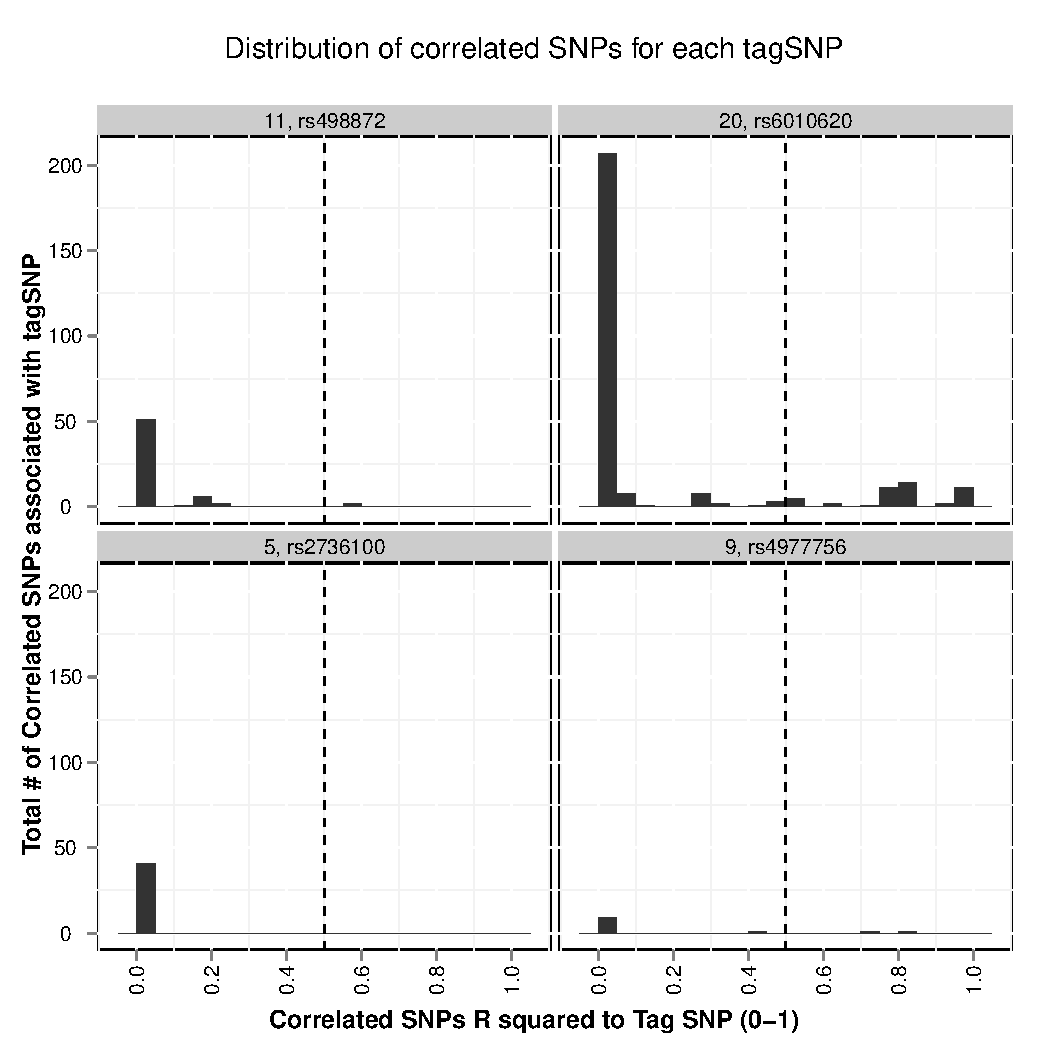
\includegraphics{glioma_dist_bysnp.pdf}
\caption{\label{fig:glioma_dist_bysnp.pdf} Distribution of Rsquare values of all
 Func-y-SNPs divided by the tagSNP and by its genomic location.}
{\footnotesize{}}
\end{center}
\end{figure}

Using `genomicSum' argument set to `TRUE' will output the overall genomic
distribution of the newly identified Func-y-SNPs (Figure
\ref{fig:glioma_genomic_sum_rcut.pdf}).  Using 'rsq' value, the plot is divided
into all Func-y-SNPs vs subset. This type of plot informs the relative
enrichment for genomic features.

\begin{Schunk}
\begin{Sinput}
> pdf("glioma_genomic_sum_rcut.pdf")
> FunciSNPplot(glioma.anno, rsq=0.5, genomicSum=TRUE, save=FALSE)
> dev.off()
\end{Sinput}
\begin{Soutput}
X11cairo 
       2 
\end{Soutput}
\end{Schunk}

\begin{figure}[ht!]
\begin{center}
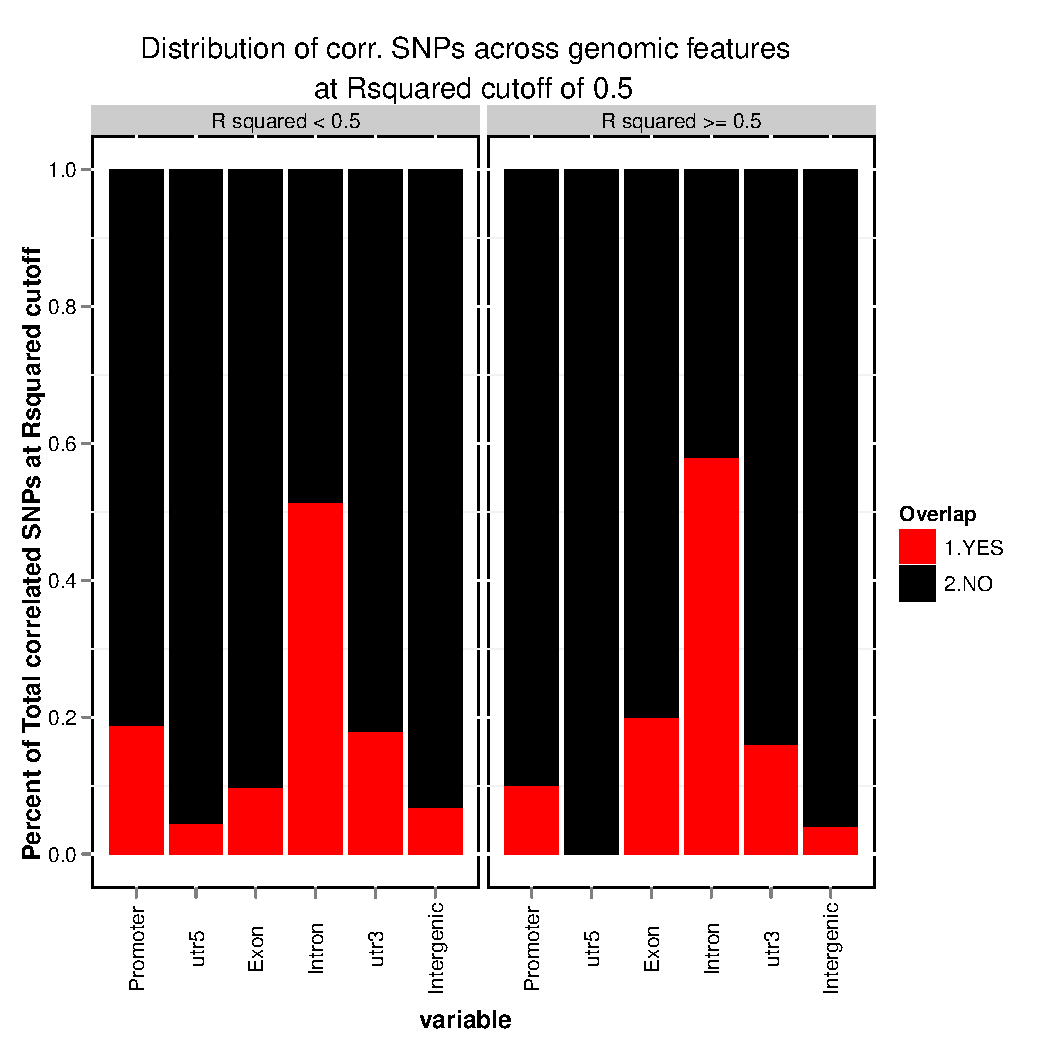
\includegraphics{glioma_genomic_sum_rcut.pdf}
\caption{\label{fig:glioma_genomic_sum_rcut.pdf} Stacked bar chart summarizing 
all correlated SNPs for each of the identified genomie features: exon, intron, 
5UTR, 3UTR, promoter, lincRNA or in gene desert. Rsquare cutoff
 at 0.5. This plot is most informative if used with a rsq value.}
{\footnotesize{}}
\end{center}
\end{figure}

Figure \ref{fig:glioma_genomic_sum_rcut.pdf} illustrates the distribution of the
Func-y-SNP by genomic features. It is clear by using an Rsquare cutoff of 0.5,
there is a slight enrichment of Func-y-SNP in introns and exonds and a depletion
at promoters and other coding regions as well as intergentic regions.

\begin{Schunk}
\begin{Sinput}
> ## Following will output a series of plots for each biofeature at rsq=0.5
> FunciSNPplot(glioma.anno, tagSummary=TRUE, rsq=0.5)
\end{Sinput}
\begin{Soutput}
Finished plotting  1 / 3 
Finished plotting  2 / 3 
Finished plotting  3 / 3 
\end{Soutput}
\end{Schunk}

Using `tagSummary' argument will automatically save all plots in a specific
folder. This is done because this function will generate a summary plot for each
biofeature. The first plot (Figure \ref{fig:TFBS_Pol2_U87_R2vsDist_riskSNP.pdf})
is a scatter plot showing the relationship between Rsquare and Distance to
tagSNP for each Func-y-SNP. 

\begin{figure}[ht!]
\begin{center}
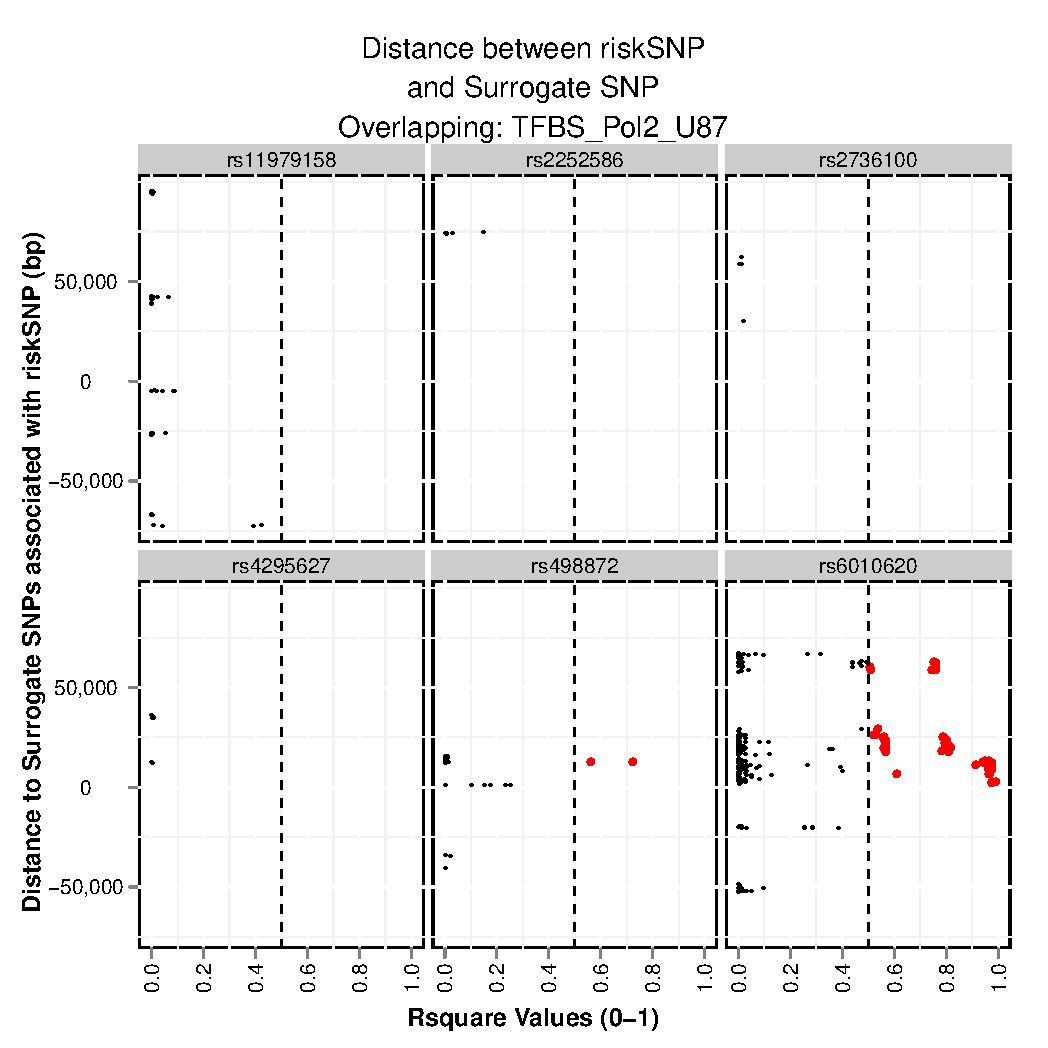
\includegraphics{FunciSNP.0.1.8/plots/TFBS_Pol2_U87_R2vsDist_riskSNP.pdf}
\caption{\label{fig:TFBS_Pol2_U87_R2vsDist_riskSNP.pdf} Scatter plot 
showing the relationship between Rsquare and Distance to tagSNP for each 
FuncySNP}
{\footnotesize{}}
\end{center}
\end{figure}

Figure \ref{fig:TFBS_Pol2_U87_R2vsDist_riskSNP.pdf} helps identify the relative
postion of all newly identified Func-y-SNP to the associated tagSNP. As
hiighlighted in figure \ref{fig:TFBS_Pol2_U87_R2vsDist_riskSNP.pdf}, it si clear
that tagSNP `rs6010620' contains many more Func-y-SNP with Rsquares $\ge$ 0.5,
and the majority of them are within 40,000 base pairs of the tagSNP. There are a
few Func-y-SNP which are more than 50,000 base pairs away while some are within
5,000 base pairs.

The second plot (Figure \ref{fig:TFBS_Pol2_U87_R2summary_riskSNP.pdf}) is a
histogram distribution of total number of Func-y-SNPs at each Rsquare value.
This plot is similar to Figure \ref{fig:glioma_dist_bysnp.pdf}, except it is
further divided by biofeature. Each set of plot is further divided by tagSNP to help identify locus with the most identifiable Func-y-SNP. This argument is best used in conjunction with a 'rsq' value.

\begin{figure}[ht!]
\begin{center}
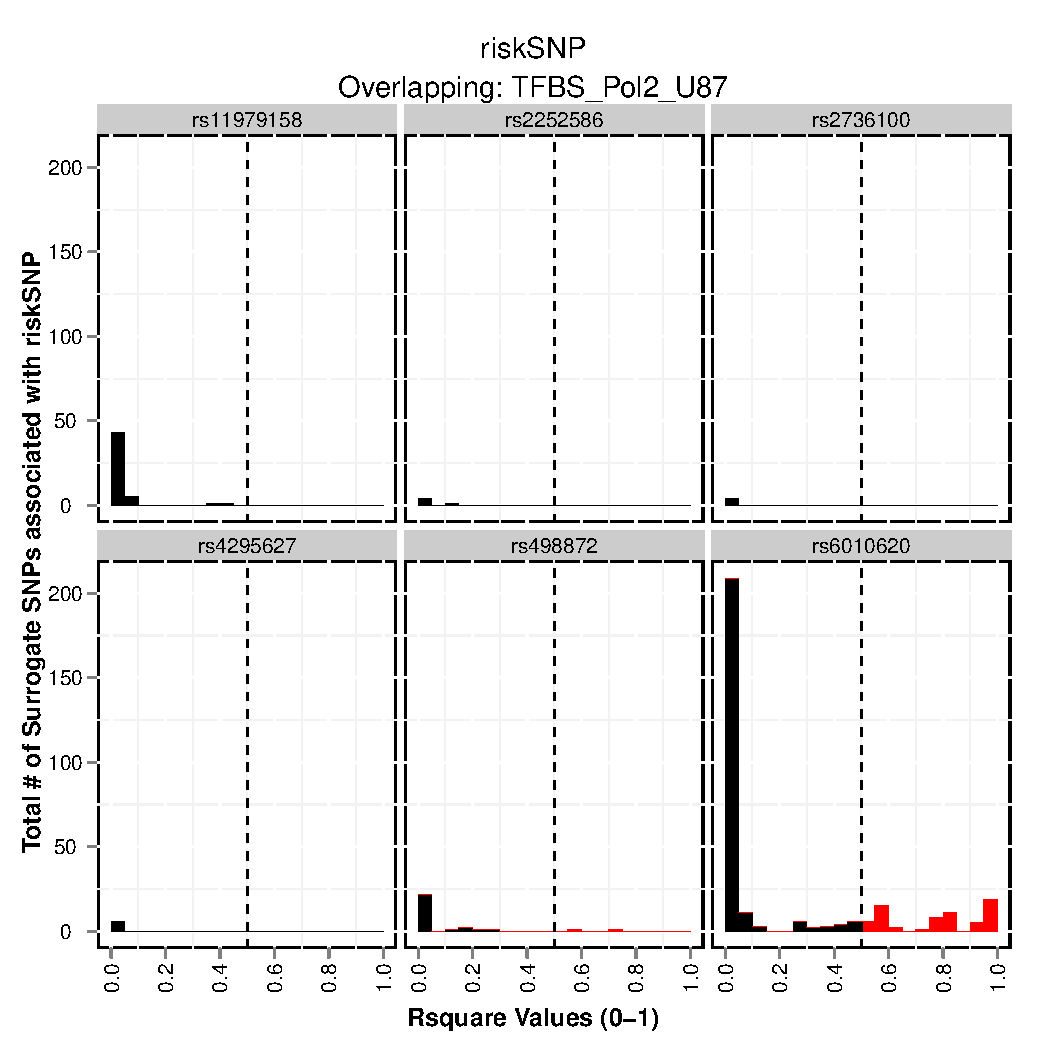
\includegraphics{FunciSNP.0.1.8/plots/TFBS_Pol2_U87_R2summary_riskSNP.pdf}
\caption{\label{fig:TFBS_Pol2_U87_R2summary_riskSNP.pdf} Histogram 
distribution of number of correlated SNPs at each Rsquare value}
{\footnotesize{}}
\end{center}
\end{figure}

\newpage


%%%%%%%%%%%%%%%%%%%%%%%%%%%%%%%%%%%%%%%%%%%%%%
%%%%%%%%%%%%%%%%%%%%%%%%%%%%%%%%%%%%%%%%%%%%%%
\section{Visualize FunciSNP results in a genomic browser (outputs BED format)}
%%%%%%%%%%%%%%%%%%%%%%%%%%%%%%%%%%%%%%%%%%%%%%
%%%%%%%%%%%%%%%%%%%%%%%%%%%%%%%%%%%%%%%%%%%%%%

Finally, after evaluating all results using the above tables and plots
functions, a unique pattern emerges that helps identify a unique cluster of
tagSNP and biofeature that can identify a set of Func-y-SNPs. To better
visualize and to get a better perspective of the location of each newly
identified Func-y-SNP, the results can be outputted using \Rmethod{FunciSNPbed}.

\Rmethod{FunciSNPbed} outputs a unique BED file which can be used to view in any
genomic browser which supports BED formats. To learn more about BED formats, see
UCSC Genome Browser FAQ (\url{http://genome.ucsc.edu/FAQ/FAQformat}). 

\begin{Schunk}
\begin{Sinput}
> ## will output to current working directory.
> FunciSNPbed(glioma.anno, rsq=0.5);
\end{Sinput}
\begin{Soutput}
Total corSNP (RED):  44 
Total tagSNP (BLK):  3 
\end{Soutput}
\begin{Sinput}
> # FunciSNPbed(rs6010620, rsq=0.5);
\end{Sinput}
\end{Schunk}

Each tagSNP which is in LD to a corresponding Func-y-SNP overlapping at least
one biofeature is colored black, while the Func-y-SNP is colored red. The
initial position is provided by the first tagSNP and the first linked
Func-y-SNP. We recommend using UCSC genome browser to view your BED files. This
is useful so you can view all public and private tracks in relation to FunciSNP
results.


%%%%%%%%%%%%%%%%%%%%%%%%%%%%%%%%%%%%%%%%%%%%%%
%%%%%%%%%%%%%%%%%%%%%%%%%%%%%%%%%%%%%%%%%%%%%%
\section{Contact information}
%%%%%%%%%%%%%%%%%%%%%%%%%%%%%%%%%%%%%%%%%%%%%%
%%%%%%%%%%%%%%%%%%%%%%%%%%%%%%%%%%%%%%%%%%%%%%
Questions or comments, please contact Simon G. Coetzee (scoetzee NEAR gmail 
 POINT com) or Houtan Noushmehr (houtana NEAR gmail POINT com).

%%%%%%%%%%%%%%%%%%%%%%%%%%%%%%%%%%%%%%%%%%%%%%
%%%%%%%%%%%%%%%%%%%%%%%%%%%%%%%%%%%%%%%%%%%%%%
\section{sessionInfo}                                                            
%%%%%%%%%%%%%%%%%%%%%%%%%%%%%%%%%%%%%%%%%%%%%%
%%%%%%%%%%%%%%%%%%%%%%%%%%%%%%%%%%%%%%%%%%%%%%

\begin{itemize}\raggedright
  \item R version 2.14.1 (2011-12-22), \verb|x86_64-pc-linux-gnu|
  \item Locale: \verb|LC_CTYPE=en_US.UTF-8|, \verb|LC_NUMERIC=C|, \verb|LC_TIME=en_US.UTF-8|, \verb|LC_COLLATE=en_US.UTF-8|, \verb|LC_MONETARY=en_US.UTF-8|, \verb|LC_MESSAGES=en_US.UTF-8|, \verb|LC_PAPER=C|, \verb|LC_NAME=C|, \verb|LC_ADDRESS=C|, \verb|LC_TELEPHONE=C|, \verb|LC_MEASUREMENT=en_US.UTF-8|, \verb|LC_IDENTIFICATION=C|
  \item Base packages: base, datasets, graphics, grDevices, grid,
    methods, splines, stats, tools, utils
  \item Other packages: annotate~1.32.1, AnnotationDbi~1.16.11,
    Biobase~2.14.0, biomaRt~2.10.0, Biostrings~2.22.0, bit~1.1-8,
    bitops~1.0-4.1, BSgenome~1.22.0,
    BSgenome.Ecoli.NCBI.20080805~1.3.17, caTools~1.12,
    ChIPpeakAnno~2.2.0, DBI~0.2-5, ff~2.2-5, FunciSNP~0.1.8,
    gdata~2.8.2, genefilter~1.36.0, GenomicFeatures~1.6.7,
    GenomicRanges~1.6.6, GGBase~3.14.0, ggplot2~0.8.9, GGtools~4.0.0,
    GO.db~2.6.1, gplots~2.10.1, gtools~2.6.2, IRanges~1.12.5,
    KernSmooth~2.23-7, lattice~0.20-0, limma~3.10.2, Matrix~1.0-3,
    multtest~2.10.0, org.Hs.eg.db~2.6.4, plyr~1.7.1, proto~0.3-9.2,
    RCurl~1.9-5, reshape~0.8.4, Rsamtools~1.6.3, RSQLite~0.11.1,
    rtracklayer~1.14.4, snpStats~1.4.1, survival~2.36-10,
    TxDb.Hsapiens.UCSC.hg19.knownGene~2.6.2, VariantAnnotation~1.0.5
  \item Loaded via a namespace (and not attached): digest~0.5.1,
    MASS~7.3-16, parallel~2.14.1, XML~3.9-4, xtable~1.6-0,
    zlibbioc~1.0.0
\end{itemize}
\end{document}
